\subsection{Compressor e Expansor}
\begin{frame}%[allowframebreaks]
  \frametitle{Compressor e Expansor}
  Podemos utilizar compressor e expansor para implementar um quantizador não uniforme.

  \begin{description}
  \item[compressor] é feito para amplificar os sinais de baixa amplitude, às custas de atenuar os sinais de alta amplitude;
  \item[expansor] faz o inverso.
  \end{description}

  \begin{figure}[h!]
  \centering
  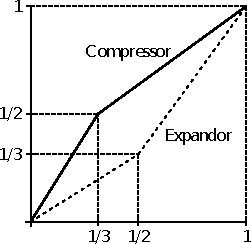
\includegraphics[width=0.3\textwidth]{images/compressor.pdf}
  \caption{Exemplo de compressor e expansor \citep{tokunbo}.}
  \label{fig:compressor}
  \end{figure}
\end{frame}


\begin{frame}[allowframebreaks]
  \frametitle{Performance do Quantizador Não Uniforme}

  O erro médio quadrático devido à quantização é dado pela Equação \ref{eq-sqnr-quants3}, repetida a seguir,
  \begin{equation} 
  \sigma_q^2 = \frac{1}{12} \sum_{k=1}^{M} p_k \Delta_k^2  , \nonumber
  \end{equation}
  onde $p_k = \Pr(t_{k-1} < x \leq t_k)$ e $\Delta_k = (t_k - t_{k-1})$.

  Suponha que o compressor apresentado na Figura \ref{fig:excompressor} seja utilizado.
  \begin{figure}[h!]
  \centering
  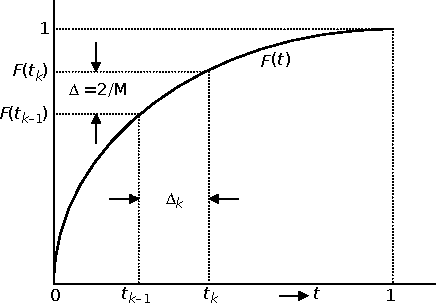
\includegraphics[width=0.6\textwidth]{images/excompressor.pdf}
  \caption{Exemplo de compressor \citep{tokunbo}.}
  \label{fig:excompressor}
  \end{figure}

  Os limiares $t_{k-1}$ e $t_{k}$, correspondentes a um codificador não uniforme, são mapeados 
  através da função compressora $F(\cdot)$ nos limiares $F(t_{k-1})$ e $F(t_k)$, uniformemente espaçados.
  Supondo o sinal no intervalo $[-1,+1]$, teremos $\Delta = 2/M$, o passo do codificador uniforme.
  Conhecendo $\Delta$ e a derivada (inclinação) de $F(t)$ no intervalo $[t_{k-1},t_{k}]$, podemos 
  determinar $\Delta_k$,
  \begin{equation}\label{eq-dk-F}
  \Delta_k = \frac{\Delta}{F'(t_k^{\ast})} = \frac{2}{M F'(t_k^{\ast})}, \quad t_{k-1} < t_k^\ast < t_k .
  \end{equation} 

  Substituindo $\Delta_k$ na Equação \ref{eq-sqnr-quants3}, teremos
  \begin{equation} \label{eq-sqnr-q-nu}
  \sigma_q^2 = \frac{1}{3} \sum_{k=1}^{M} \frac{p_k}{M^2 (F'(t_k^{\ast}))^2} , \quad t_{k-1} < t_k^\ast < t_k .
  \end{equation}

  Se o número de níveis $M$ for grande, o somatório em \ref{eq-sqnr-q-nu} poderá ser aproximado por
  uma integral:
  \begin{equation} \label{eq-sqnr-q-nu2}
  \sigma_q^2 = \frac{1}{3M^2} \int_{-1}^{+1} \frac{p(x)}{ (F'(x))^2 } \mathrm{d}x = \frac{2}{3M^2} \int_{0}^{+1} \frac{p(x)}{ (F'(x))^2 } \mathrm{d}x  ,
  \end{equation}
  onde utilizamos a simplificação em que a $p(x)$ é simétrico par.

  Para um sinal com excursão entre $-X_m$ e $+X_m$, teremos
  \begin{equation} \label{eq-sqnr-q-nu2}
  \sigma_q^2 = \frac{2 X_m^2}{3M^2} \int_{0}^{X_m} \frac{p(x)}{ (F'(x))^2 } \mathrm{d}x  .
  \end{equation} 

\end{frame}

\begin{frame}[allowframebreaks]
  \frametitle{Compressão Logarítmica}
  Em um sistema de telecomunicações, desejamos uma SNR constante, independente da distribuição do sinal de entrada.
  Desejamos então encontrar o compressor $F$ que alcança este objetivo.

  \begin{equation} \label{eq-sqnr-log-const}
  \textmd{SNR} = \frac{\sigma_x^2}{\sigma_q^2} = \frac{2 \int_0^1 x^2 p(x) \mathrm{d}x}{ \frac{2}{3M^2} \int_0^1 \frac{p(x)}{(F'(x))^2} \mathrm{d}x } .
  \end{equation}
  A expressão em \ref{eq-sqnr-log-const} pode ser feita constante escolhendo
  \begin{equation} \label{eq-dcompr}
  F'(x) = \frac{k^{-1}}{x} ,
  \end{equation}
  com parâmetro $k$ a ser especificado.

  A curva de compressão $F(x)$ é obtida realizando-se a integração e escolhendo a constante de integração 
  para que a condição de contorno $F(1)=1$ seja satisfeita, obtendo assim
  \begin{equation} \label{eq-compr}
  F(x) = 1 + k^{-1} \ln x .
  \end{equation}
  Para este caso a SNR obtida será
  \begin{equation} \label{eq-sqnr-log-const2}
  \textmd{SNR} =  \frac{3M^2}{k^2} .
  \end{equation}
  Para sinal com extensão de $-X_m$ a $X_m$, teremos
  \begin{equation} \label{eq-compr2}
  F(x) = X_m + k^{-1} \ln \left(\frac{x}{X_m}\right) .
  \end{equation}

  \begin{figure}[h!]
  \centering
  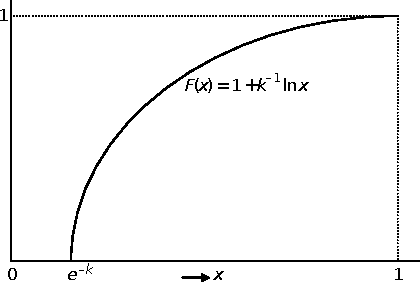
\includegraphics[width=0.6\textwidth]{images/Fx.pdf}
  \caption{Gráfico de $F(x) = 1 + k^{-1} \ln x$ \citep{tokunbo}.}
  \label{fig:Fx}
  \end{figure}

  Através da Equação \ref{eq-dk-F} e da escolha feita em \ref{eq-dcompr}, podemos verificar
  que o tamanho do passo de quantização é proporcional à amplitude do sinal, quando utilizamos
  a compressão logarítmica dada por $F(x) = 1 + k^{-1} \ln x$. 
  \begin{equation}
  \Delta_k = \frac{2}{M F'(t_k^{\ast})} = \frac{2}{M k^{-1}} t_k^{\ast} .
  \end{equation}
  Para valores próximo da origem,
  esta proporcionalidade não poderá ser mantida, pois $\ln x$ diverge
  quando $x \rightarrow 0$.

  Uma lei de compressão prática não pode ter tal descontinuidade, devendo também especificar a compressão
  dada a sinais de baixa amplitude.
\end{frame}

\begin{frame}[allowframebreaks]
  \frametitle{lei $\mu$}
   Esta aproximação desloca o cruzamento com zero de $F(x)$, 
   que ocorria em $x = e^{-k}$, para a origem.

   \begin{equation}
   F(x) = \frac{\log (1 + \mu x)}{ \log (1 + \mu)} , \quad 0 \leq x \leq 1 ,
   \end{equation}
   onde a base do logaritmo é irrelevante.

  \begin{equation}
   F(x) = \sign (x) \frac{\log (1 + \mu |x|)}{ \log (1 + \mu)} , \quad -1 \leq x \leq 1 .
  \end{equation}

  \framebreak

  Note que, quando $\mu \gg 1$, esta lei aproxima uma curva logaritma para valores grandes.
  \begin{equation}
  F(x) = \frac{\log (1 + \mu x)}{\log(1+\mu)} \approx \frac{\log(\mu x)}{\log(\mu)} = 1 + \frac{\log(x)}{\log(\mu)} = 1 + \frac{\ln x}{\ln \mu} .
  \end{equation}
  Teremos então $k = \ln \mu$ e assim a SNR para sinais grandes será aproximadamente $3M^2/(\ln \mu)^2$.

  \framebreak

  \begin{figure}[h!]
  \centering
  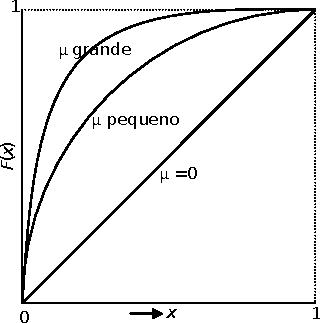
\includegraphics[width=0.4\textwidth]{images/mulaw.pdf}
  \caption{Curva de compressores segundo a lei $\mu$ \citep{tokunbo}.}
  \label{fig:mulaw}
  \end{figure}
  
  A lei $\mu$ é utilizada no padrão ITU G.711 PCM através de uma aproximação discreta usando $\mu=255$.
\end{frame}

\begin{frame}[allowframebreaks]
  \frametitle{lei A}

  \begin{figure}[h!]
  \centering
  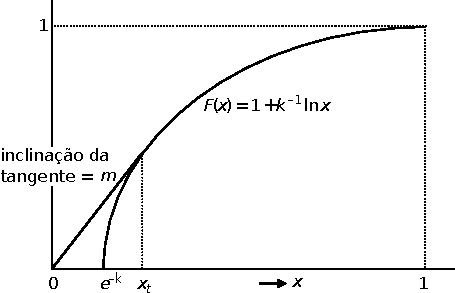
\includegraphics[width=0.6\textwidth]{images/Alaw.pdf}
  \caption{Curva de compressores segundo a lei A \citep{tokunbo}.}
  \label{fig:Alaw}
  \end{figure}

  \begin{equation}
  k = 1 + \ln A .
  \end{equation}

  \begin{equation}
  F(x) = \begin{cases}
  \frac{Ax}{1+\ln A} , \quad 0 \leq x \leq 1/A , \\
  \frac{1+\ln Ax}{1+\ln A}, \quad 1/A \leq x \leq 1 .
  \end{cases}
  \end{equation}

  \bibentry{tokunbo}
  %\printbibliography[keyword={tokunbo},title={Mais informações:}]
\end{frame}

